\chapter{基于原模图构造的LDPC码}
\section{LDPC码的原模图及LDPC码的叠加方式}
许多好的LDPC码都是通过人工叠加短LDPC码而形成的。
LDPC码的叠加能很形象地通过Tanner图的方式表现出来。
考虑一个短LDPC码,以及与其对应的小的Tanner图,如图\ref{fig:basegraph}。
这个小的Tanner图有多个名字,如原模图、基本图或者投影图。
从原模图、基本图这两个名字可以看出,这种小的Tanner图是组成更大的Tanner图的基础。
而投影图这个名字则说明了,这个小的Tanner图是叠加其自身而构成更大的Tanner图的投影。
图\ref{fig:basegraph}中圈中等号代表变量节点,圈中加号代表校验节点,该图右侧为对应LDPC码的校验矩阵。
\begin{center}
\def\check{%
    \filldraw [fill=white,very thick] (0,0) circle (5pt);
    \draw [very thick] (0,3.5pt)--(0,-3.5pt);
    \draw [very thick] (3.5pt,0)--(-3.5pt,0);
}
\def\bit{%
    \filldraw [fill=white,very thick] (0,0) circle (5pt);
    \draw [very thick] (-3.2pt,2.2pt)--(3.2pt,2.2pt);
    \draw [very thick] (-3.2pt,-2.2pt)--(3.2pt,-2.2pt);
}
\begin{tikzpicture}
\draw [very thick] (-3,2.5) -- (-2,0);
\draw [very thick] (3,2.5) -- (-2,0);
\draw [very thick] (-1,2.5) -- (0,0);
\draw [very thick] (1,2.5) -- (0,0);
\draw [very thick] (-3,2.5) -- (2,0);
\draw [very thick] (-1,2.5) -- (2,0);
\draw [very thick] (1,2.5) -- (2,0);
\draw [very thick] (3,2.5) -- (2,0);
\begin{scope}[xshift=1cm,yshift=2.5cm]
\bit
\end{scope}
\begin{scope}[xshift=-1cm,yshift=2.5cm]
\bit
\end{scope}
\begin{scope}[xshift=3cm,yshift=2.5cm]
\bit
\end{scope}
\begin{scope}[xshift=-3cm,yshift=2.5cm]
\bit
\end{scope}
\begin{scope}[xshift=2cm,yshift=0cm]
\check
\end{scope}
\begin{scope}[xshift=-2cm,yshift=0cm]
\check
\end{scope}
\check
\draw [<->,thick] (3.3,1.25) -- (4.3,1.25);
\node at (7,1.25) (steptwo){
	\begin{minipage}{0.40\textwidth}
		\begin{equation*}
    H_b = \left(
      \begin{array}{cccc}
        1 & 0 & 0 & 1 \\
        0 & 1 & 1 & 0 \\
        1 & 1 & 1 & 1 
      \end{array} \right)
\end{equation*}
	\end{minipage}
};
\end{tikzpicture}
\figurecaption{基本图}
\label{fig:basegraph}
\end{center}

对于规则的LDPC码,可以采取更简单的原模图来描述。由于规则的LDPC码的每一个信息节点与校验节点都有相同的度分布,即相同的边连接模式,所以我们可以将基本图折叠起来,让它变成如图\ref{fig:protograph}的形状。图\ref{fig:protograph}表示的是(3,6)正则LDPC码的原模图以及其对应的基本矩阵描述。
\begin{center}
\def\linkdoub{\draw [double distance=1mm, very thick] (0,0)--}
\def\linksing{\draw [very thick] (0,0)--}
\def\check{%
    \filldraw [fill=white,very thick] (0,0) circle (5pt);
    \draw [very thick] (0,3.5pt)--(0,-3.5pt);
    \draw [very thick] (3.5pt,0)--(-3.5pt,0);
}
\def\bit{%
    \filldraw [fill=white,very thick] (0,0) circle (5pt);
    \draw [very thick] (-3.2pt,2.2pt)--(3.2pt,2.2pt);
    \draw [very thick] (-3.2pt,-2.2pt)--(3.2pt,-2.2pt);
}
\def\thetaone{90}
\def\thetatwo{-90}
\def\armLength{0.9}
\def\symbolDist{1}
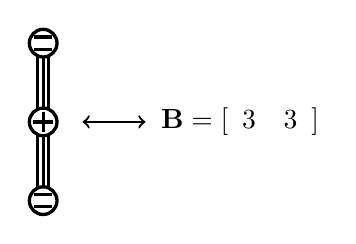
\begin{tikzpicture}
\linkdoub(\thetaone:\armLength);
\linksing(\thetaone:\armLength);
\linksing(\thetatwo:\armLength);
\begin{scope}[shift=(\thetaone:\symbolDist)]
\bit
\end{scope}
\begin{scope}[shift=(\thetatwo:\symbolDist)]
\linkdoub(\thetaone:\armLength);
\linksing(\thetaone:\armLength);
\bit
\end{scope}
\check
\draw [<->,thick] (0.5,0) -- (1.3,0);
\node [align=center] at (2.5,0) {$ \mathbf{B} = [\begin{array}{cc} 3&3 \end{array}]$};

\end{tikzpicture}
\figurecaption{LDPC码的原模图}
\label{fig:protograph}
\end{center}

为了构造有结构的LDPC码,首先要将图\ref{fig:basegraph}复制m次。
此时变量节点、校验节点以及节点间相连的边都变成了m份,形成了一个簇状的Tanner图,如图\ref{fig:copy}。
\begin{center}
\def\check{%
    \filldraw [fill=white,very thick] (0,0) circle (5pt);
    \draw [very thick] (0,3.5pt)--(0,-3.5pt);
    \draw [very thick] (3.5pt,0)--(-3.5pt,0);
}
\def\bit{%
    \filldraw [fill=white,very thick] (0,0) circle (5pt);
    \draw [very thick] (-3.2pt,2.2pt)--(3.2pt,2.2pt);
    \draw [very thick] (-3.2pt,-2.2pt)--(3.2pt,-2.2pt);
}
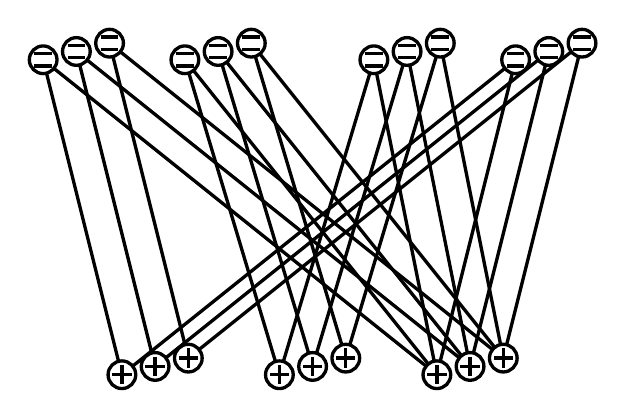
\begin{tikzpicture}
\foreach \x / \z in {0/0,12/3,24/6}
{
\begin{scope}[xshift=\x,yshift=\z]
	\draw[very thick] (-3,4) -- (-2,0);
	\draw[very thick] (3,4) -- (-2,0);
	\draw[very thick] (-1.2,4) -- (0,0);
	\draw[very thick] (1.2,4) -- (0,0);
	\draw[very thick] (-3,4) -- (2,0);
	\draw[very thick] (-1.2,4) -- (2,0);
	\draw[very thick] (1.2,4) -- (2,0);
	\draw[very thick] (3,4) -- (2,0);
\begin{scope}[xshift=1.2cm,yshift=4cm]
\bit
\end{scope}
\begin{scope}[xshift=-1.2cm,yshift=4cm]
\bit
\end{scope}
\begin{scope}[xshift=3cm,yshift=4cm]
\bit
\end{scope}
\begin{scope}[xshift=-3cm,yshift=4cm]
\bit
\end{scope}
\begin{scope}[xshift=2cm,yshift=0cm]
\check
\end{scope}
\begin{scope}[xshift=-2cm,yshift=0cm]
\check
\end{scope}
\check
\end{scope}
}
\end{tikzpicture}
\figurecaption{复制m次基本图}
\label{fig:copy}
\end{center}

原模图被复制了m次之后,虽然变量节点、校验节点以及节点间相连的边都变成了m份,
但是此时这m个原模图还是隔离的。
所以要对每一个边的簇应用置换方法,使得不同的原模图之间相连起来。
此时便完成了从原模图构造如原模图m倍大小的有结构的LDPC码,如图\ref{fig:structed}。

如果采用矩阵的表述方式,一开始我们有一个LDPC短码的校验矩阵$H_b$,如图\ref{fig:basegraph}的右边的矩阵所示。
令$\mathcal{P}$为$m\times m$维置换矩阵的集合。
我们通过把$H_b$中的每个元素换成$m\times m$的矩阵来形成$m$倍大的LDPC码。
其中,把$H_b$中为$1$的元素换成$\mathcal{P}$中的某个矩阵,把$H_b$中为$0$的元素换成零矩阵。
通过这种复制方式,LDPC短码的校验矩阵$H_b$变成了$m$倍大的校验矩阵:
\begin{equation}
    H = \left(
      \begin{array}{cccc}
        P^2 & 0 & 0 & P^1 \\
        0 & P^3 & P^1 & 0 \\
        P^1 & P^3 & P^2 & P^2 
      \end{array} \right)
\end{equation}

其中$P^i$对应循环置换矩阵,其意义是对集合$\{1,\dots,m\}$进行移位操作$i-1$次:
它的列向量对应于变量节点,行向量对应于校验节点。比如$P^1$对应单位矩阵,以及
\begin{equation}
    P^2 = \left(
      \begin{array}{ccc}
        0 & 0 & 1 \\
        1 & 0 & 0 \\
        0 & 1 & 0
      \end{array} \right)
\end{equation}

$P^2$表示的意思是将第一个原模图的第一个变量节点连接到第二个原模图的第一个校验节点,将第二个原模图的第一个变量节点连接到第三个原模图的第一个校验节点,将第三个原模图的第一个变量节点连接到第一个原模图的第一个校验节点。
\begin{center}
\def\check{%
    \filldraw [fill=white,very thick] (0,0) circle (5pt);
    \draw [very thick] (0,3.5pt)--(0,-3.5pt);
    \draw [very thick] (3.5pt,0)--(-3.5pt,0);
}
\def\bit{%
    \filldraw [fill=white,very thick] (0,0) circle (5pt);
    \draw [very thick] (-3.2pt,2.2pt)--(3.2pt,2.2pt);
    \draw [very thick] (-3.2pt,-2.2pt)--(3.2pt,-2.2pt);
}
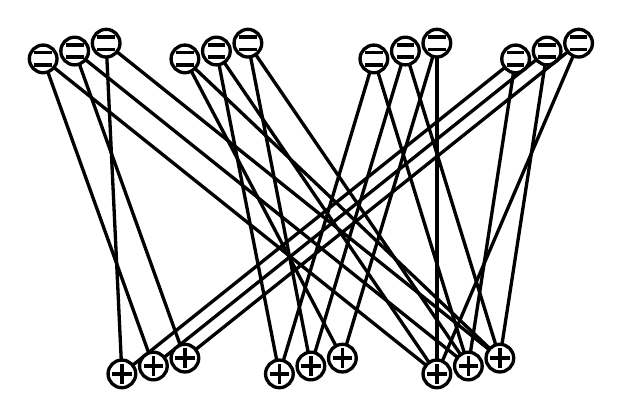
\begin{tikzpicture}
%p2
  \draw[very thick] (-2.2,4.2) -- (-2,0);
  \draw[very thick] (-3,4) -- (-1.6,0.1);
  \draw[very thick] (-2.6,4.1) -- (-1.2,0.2);
%p3
  \draw[very thick] (-0.8,4.1) -- (0,0);
  \draw[very thick] (-0.4,4.2) -- (0.4,0.1);
  \draw[very thick] (-1.2,4) -- (0.8,0.2);
%p3
  \draw[very thick] (-0.8,4.1) -- (2,0);
  \draw[very thick] (-0.4,4.2) -- (2.4,0.1);
  \draw[very thick] (-1.2,4) -- (2.8,0.2);
%p2
  \draw[very thick] (2.0,4.2) -- (2,0);
  \draw[very thick] (1.2,4) -- (2.4,0.1);
  \draw[very thick] (1.6,4.1) -- (2.8,0.2);
%p2
  \draw[very thick] (3.8,4.2) -- (2,0);
  \draw[very thick] (3,4) -- (2.4,0.1);
  \draw[very thick] (3.4,4.1) -- (2.8,0.2);
\foreach \x / \z in {0/0,0.4/0.1,0.8/0.2}
{
\begin{scope}[xshift=\x cm,yshift=\z cm]
\draw[very thick] (3,4) -- (-2,0);
\draw[very thick] (1.2,4) -- (0,0);
\draw[very thick] (-3,4) -- (2,0);
\begin{scope}[xshift=1.2cm,yshift=4cm]
\bit
\end{scope}
\begin{scope}[xshift=-1.2cm,yshift=4cm]
\bit
\end{scope}
\begin{scope}[xshift=3cm,yshift=4cm]
\bit
\end{scope}
\begin{scope}[xshift=-3cm,yshift=4cm]
\bit
\end{scope}
\begin{scope}[xshift=2cm,yshift=0cm]
\check
\end{scope}
\begin{scope}[xshift=-2cm,yshift=0cm]
\check
\end{scope}
\check
\end{scope}
}
\end{tikzpicture}
\figurecaption{具有一定结构的LDPC码}
\label{fig:structed}
\end{center}

\section{LDPC分组码的构造}
设计码率为$R=b/c$的LDPC分组码的原模图有$c$个变量节点和$c-b$个校验节点。
它能生成不同码长的,设计码率为$R$,有相同的度分布的分组码。
一个有$c=2$个变量节点,变量节点的度为3,和$c-b=1$个校验节点,校验节点的度为6的分组码原模图的例子可以参看图\ref{fig:basegraph}。

下面将描述$q$元LDPC分组码的构造方法。
GF($q$)为含$q=2^m$个元素的有限域,其中$m$为在GF($q$)代表一个符号所需的位数。
令$M$为原模图叠加数,其中$M$是一个大整数。
通过以下两步从原模图的$(c-b)\times c$邻接矩阵$\mathbf{B}=[B_{i,j}]$构造码长为$n_{BC}=Mc$的$q$元LDPC分组码:
\begin{enumerate}
\item 将$\mathbf{B}$中的非零元$B_{i,j}$替换为随机选择的$M \times M$置换矩阵,将$\mathbf{B}$中的零元$B_{i,j}$替换为$M \times M$零矩阵。此时得到对应于$\mathbf{B}$的二元校验矩阵$\mathbf{H}$;
\item 将$\mathbf{H}$中非零元替换为从有限域GF($q$)中随机选取的元素,得到LDPC分组码的$q$元校验矩阵$\mathbf{H}_{BC}$。
\end{enumerate}
对于LDPC分组码,必须等待整个码块接受完毕才能执行置信传播解码算法。故$q$元LDPC分组码的解码延时为
\begin{equation}
T_{BC}=n_{BC}\cdot m = Mmc
\end{equation}

\section{LDPC卷积码的构造}

对于给定码率为$R=b/c$的LDPC卷积码,其定义为,存在校验矩阵$\mathbf{H}_{[\infty]}$使得无限长向量$\mathbf{v}_{[\infty]}$有$\mathbf{H}_{[\infty]}\mathbf{v}_{[\infty]}^\text{T} =\mathbf{0}_{[\infty]}$,其中
\begin{equation}
    \mathbf{H}_{[\infty]} = \left[
          \begin{array}{ccccc}
            \mathbf{H}_0(1) & & & & \\
            \mathbf{H}_1(1) & \mathbf{H}_0(2) & & & \\
            \vdots & \mathbf{H}_1(2) & \ddots & & \\
            \mathbf{H}_{m_s}(1) & \vdots & \ddots & \mathbf{H}_0(t) & \\
             & \mathbf{H}_{m_s}(2) & \ddots & \mathbf{H}_1(t) & \ddots\\
             & & \ddots & \vdots & \ddots \\
             & & & \mathbf{H}_{m_s}(t) & \ddots \\
             & & & & \ddots
          \end{array} \right]
\end{equation}
而$\mathbf{0}_{[\infty]}$是无限长零向量。
$\mathbf{H}_i(t),i=0,1,\dots,m_s$为$(c-b)\times c$的矩阵满足以下条件:
\begin{itemize}
\item $\mathbf{H}_i(t)=\mathbf{0}$,当$i<0$和$i>m_s$,$\forall t \geq 1$;
\item $\exists t\geq 0$,使得$\mathbf{H}_{m_s}(t) \neq \mathbf{0}$;
\item $\forall t \geq 1$,$\mathbf{H}_0(1)$满秩。
\end{itemize}

其中参数$m_s$称为LDPC卷积码的记忆因子。
$\nu = (m_s+1)c$为LDPC卷积码的限制长度。
对于$\forall t,\tau>1,\mathbf{H}_i(t) = \mathbf{H}_i(t+\tau),\forall i = 0,1,\dots,m_s$的情况,我们称LDPC卷积码具有周期性。
若$\tau=1$,称LDPC卷积码为时不变的。
另外,截尾的LDPC卷积码的校验矩阵长度有限,即在$L$时刻终止,如
\begin{equation}
    \mathbf{H}_{[L]} = \left[
          \begin{array}{cccc}
            \mathbf{H}_0(1) & & & \\
            \mathbf{H}_1(1) & \mathbf{H}_0(2) & & \\
            \vdots & \mathbf{H}_1(2) & \ddots & \\
            \mathbf{H}_{m_s}(1) & \vdots & \ddots & \mathbf{H}_0(L) \\
             & \mathbf{H}_{m_s}(2) & \ddots & \mathbf{H}_1(L) \\
             & & \ddots & \vdots \\
             & & & \mathbf{H}_{m_s}(L)
          \end{array} \right]
\end{equation}

下面通过原模图来构造截尾的时不变的LDPC卷积码。
设原模图的基本矩阵为$(c-b)\times c$的$\mathbf{B}$。
首先构造$\mathbf{B}_{CC}$
\begin{equation}
    \mathbf{B}_{CC} = \left[
          \begin{array}{ccc}
            \mathbf{B}_0& & \\
            \mathbf{B}_1 & \mathbf{B}_0 & \\
            \vdots & \mathbf{B}_1 & \ddots \\
            \mathbf{B}_{m_s} & \vdots & \ddots \\
             & \mathbf{B}_{m_s} & \ddots \\
             & & \ddots 
          \end{array} \right]
\end{equation}
其中$m_s$为在图\ref{fig:LDPCCC}中当前原模图与前一个原模图相连的边数。$\mathbf{B}_0 , \mathbf{B}_1 , \dots , \mathbf{B}_{m_s}$为$(c-b)\times c$矩阵,且满足
\begin{equation}
\sum^{m_s}_{i=0} \mathbf{B}_i = \mathbf{B}
\end{equation}

然后将$\mathbf{B}_{CC}$中的非零元替换为随机选择的$M \times M$置换矩阵,将$\mathbf{B}_{CC}$中的零元替换为$M \times M$零矩阵,得到LDPC卷积码校验矩阵$\mathbf{H}_{CC}$。
最后将$\mathbf{H}_{CC}$中的非零元替换为从有限域GF($q$)中随机选取的元素,得到LDPC卷积码的$q$元校验矩阵$\mathbf{H}_{CC}$,其限制长度为$v_s=(m_s+1)Mc$。

图\ref{fig:LDPCCC}为通过原模图叠加方法构造LDPC卷积码的示意图。
首先复制几次(3,6)正则LDPC码的原模图,设定记忆因子$m_s=1$,然后将原模图之间连接起来。
其中,原模图的基本矩阵为$ \mathbf{B} = [\begin{array}{cc} 3&3 \end{array}]$,使用到的组成矩阵为$\mathbf{B}_0 = [\begin{array}{cc} 2&1 \end{array}]$,$\mathbf{B}_1 = [\begin{array}{cc} 1&2 \end{array}]$。

\begin{center}
\def\linkdoub{\draw [double distance=1mm, very thick] (0,0)--}
\def\linksing{\draw [very thick] (0,0)--}
\def\check{%
    \filldraw [fill=white,very thick] (0,0) circle (5pt);
    \draw [very thick] (0,3.5pt)--(0,-3.5pt);
    \draw [very thick] (3.5pt,0)--(-3.5pt,0);
}
\def\bit{%
    \filldraw [fill=white,very thick] (0,0) circle (5pt);
    \draw [very thick] (-3.2pt,2.2pt)--(3.2pt,2.2pt);
    \draw [very thick] (-3.2pt,-2.2pt)--(3.2pt,-2.2pt);
}
\def\thetaone{90}
\def\thetatwo{-90}
\def\thetathree{60}
\def\thetafour{-60}
\def\armLength{0.9}
\def\symbolDist{1}
\begin{tikzpicture}
\foreach \x in {0.8,1.6,2.4,3.2,4}
{
\begin{scope}[shift=(0:\x)]
\linkdoub(\thetaone:\armLength);
\linksing(\thetaone:\armLength);
\linksing(\thetatwo:\armLength);
\begin{scope}[shift=(\thetaone:\symbolDist)]
\bit
\end{scope}
\begin{scope}[shift=(\thetatwo:\symbolDist)]
\linkdoub(\thetaone:\armLength);
\linksing(\thetaone:\armLength);
\bit
\end{scope}
\check
\end{scope}
}
\node at (4.7,0.9) {\ldots};
\node at (4.7,0) {\ldots};
\node at (4.7,-0.9) {\ldots};
\draw [->,very thick] (5.3,0) -- (6,0);
\begin{scope}[shift=(0:5.6)]
\foreach \x in {1,2,...,5}
{
	\begin{scope}[shift=(0:\x)]
		\linkdoub(\thetathree:\armLength);
		\linksing(\thetafour:\armLength);
		\check
		\begin{scope}[shift=(\thetathree:\symbolDist)]
		\linksing(\thetafour:\armLength);
		\bit
		\end{scope}
		\begin{scope}[shift=(\thetafour:\symbolDist)]
		\linkdoub(\thetathree:\armLength);
		\bit
		\end{scope}
	\end{scope}
}
\node at (6.5,0.9) {\ldots};
\node at (6.5,0) {\ldots};
\node at (6.5,-0.9) {\ldots};
\end{scope}
\end{tikzpicture}
\figurecaption{构造LDPC卷积码}
\label{fig:LDPCCC}
\end{center}

由于记忆参数$m_s=1$的LDPC卷积码有优秀的解码阈值,以及在有限长情况下,使用窗口参数较小的滑动窗口译码算法能达到较好的性能,
在之后的实证分析中,本文只考虑记忆参数$m_s=1$的LDPC卷积码。
并且本文只考虑$(d_v,d_c)$正则LDPC卷积码,即$\mathbf{H}_{CC}$中每行重量为$d_c$,每列重量为$d_v$。
这是因为$(d_v,d_c)$正则LDPC卷积码具有逼近信道容量的性能,以及其解码复杂度低于非正则LDPC卷积码。

为了公平地比较LDPC卷积码与LDPC分组码的性能,
本文限定构造LDPC卷积码与LDPC分组码的校验矩阵的方法如下。
选择两个$(c-b)\times c$矩阵$\mathbf{B}_0$和$\mathbf{B}_1$,使得$\mathbf{B}_0 + \mathbf{B}_1$为$(d_v,d_c)$正则矩阵。$(d_v,d_c)$正则LDPC分组码的基本矩阵为
\begin{equation}
    \mathbf{B}_{BC} = \left[
          \begin{array}{cc}
            \mathbf{B}_0 & \mathbf{B}_1\\
            \mathbf{B}_1 & \mathbf{B}_0
          \end{array} \right]_{2(c-b)\times 2c}
\end{equation}

其中$\mathbf{B}_{BC}$每个列向量的重量为$d_v$,每个行向量的重量为$d_c$。
然后使用第二节的原模图叠加方法构造LDPC分组码的校验矩阵
\begin{equation}
    \mathbf{H}_{BC} = \left[
          \begin{array}{cc}
            \mathbf{H}_0 & \mathbf{H}_1\\
            \mathbf{H}_1 & \mathbf{H}_0
          \end{array} \right]_{2(c-b)M \times 2cM}
\end{equation}

对于LDPC卷积码,使用相同的$\mathbf{B}_0$和$\mathbf{B}_1$,得到$(d_v,d_c)$正则LDPC卷积码的基本矩阵为
\begin{equation}
    \mathbf{B}_{CC} = \left[
          \begin{array}{ccccc}
            \mathbf{B}_0 & & & & \\
            \mathbf{B}_1 & \mathbf{B}_0 & & & \\
             & \mathbf{B}_1 & \mathbf{B}_0 & & \\
             & & \mathbf{B}_1 & \mathbf{B}_0 & \\
             & & & \mathbf{B}_1 & \ddots \\
             & & & & \ddots
          \end{array} \right]
\end{equation}
然后使用原模图叠加方法构造LDPC卷积码的校验矩阵
\begin{equation}
    \mathbf{H}_{CC} = \left[
          \begin{array}{ccccc}
            \mathbf{H}_0 & & & & \\
            \mathbf{H}_1 & \mathbf{H}_0 & & & \\
             & \mathbf{H}_1 & \mathbf{H}_0 & & \\
             & & \mathbf{H}_1 & \mathbf{H}_0 & \\
             & & & \mathbf{H}_1 & \ddots \\
             & & & & \ddots
          \end{array} \right]
\end{equation}

基于以上构造规则,可以使用其他的基本矩阵(见表\ref{table:formmatrix})构造LDPC分组码校验矩阵$\mathbf{H}_{BC}$与LDPC卷积码校验矩阵$\mathbf{H}_{CC}$。当原模图叠加数为$M$,有限域元素个数为$q=2^m$时,LDPC分组码的码长和LDPC卷积码的限制长度都等于$2Mmc$。

从LDPC卷积码的校验矩阵$\mathbf{H}_{CC}$以及LDPC分组码的校验矩阵$\mathbf{H}_{BC}$可以看出,$\mathbf{H}_{CC}$中的某一部分在周期性地重复$\mathbf{H}_{BC}$。
这种构造方式源于\parencite{782171}中,从LDPC分组码衍生LDPC卷积码的展开算法。
同时我们还可以注意到,尽管我们称由$\mathbf{H}_{CC}$生成的LDPC卷积码是$(d_v,d_c)$正则的,
但是$\mathbf{H}_{CC}$并非真正的$(d_v,d_c)$正则校验矩阵,因为它的前$(c-b)$行的重量小于$d_c$。
而正是因为$(d_v,d_c)$正则LDPC卷积码具有这种微小的结构不规则性,其解码阈值才能逼近信道容量。
\begin{center}
\tablecaption{构造LDPC分组码和LDPC卷积码的组成矩阵}
\label{table:formmatrix}
\begin{tabular}{c|c|c}
 \hline
码 & 组成矩阵 &码长/限制长度 \\ \hline
(2,4)正则 & 
$\mathbf{B}_0 = \mathbf{B}_1 = [\begin{array}{cc} 1&1 \end{array}]$ & 4Mm \\ \hline
(3,6)正则 & 
 $\mathbf{B}_0 = [\begin{array}{cc} 2&1 \end{array}]$,$\mathbf{B}_1 = [\begin{array}{cc} 1&2 \end{array}]$ & 4Mm \\ \hline
\end{tabular}
\end{center}